\documentclass[12pt]{article}


%%%%%%%%%%%%%%%%%%%%%%%%%%%%%%%%%%%%%%%%%%%%%%%%%%%%%%%%%%%%%%%%%%%%%%% 
%%%%%%%%% Packages - these are like libraries, parts of code that have already been made for you to use that are included in Overleaf.
\usepackage[english]{babel}
% \usepackage[utf8x]{inputenc}

\usepackage{tabularx}

\usepackage{csquotes}
\usepackage{algorithm2e}
\usepackage{fancyhdr}
\usepackage{graphicx}
\usepackage{subcaption}
\usepackage{mathtools}
\usepackage{parskip}
\usepackage{tkz-tab}  
\usepackage{tikz, xcolor, lipsum}
\usepackage{url}
\usepackage{hyperref}
\usepackage{vmargin}
\usepackage[framemethod=tikz]{mdframed}
\usepackage{multirow}
\usepackage[
backend=biber,
style=alphabetic,
sorting=ynt
]{biblatex}
\addbibresource{ref.bib}

\graphicspath{{images/}}
\DeclarePairedDelimiter\ceil{\lceil}{\rceil}
\DeclarePairedDelimiter\floor{\lfloor}{\rfloor}
\setmarginsrb{3 cm}{1.5 cm}{3cm}{1.5 cm}{1 cm}{1.5 cm}{1 cm}{1.5 cm}
\RestyleAlgo{ruled}


%%%%%%%%%%%%% Input the document's title, name and date here

\title{N-Body simulation}	
\author{CSE305}
\date{
    Minjoo KIM \\ 
    Nhat VO \\
    Vrushank AGRAWAL
}

%%%%%%%%%%%%%%%%%% The following lines are all just formatting ... not necessary at all if you make your own document, but it looks nice
\makeatletter
\let\thetitle\@title
\let\theauthor\@author
\let\thedate\@date
\let\thecourse\@course
\makeatother

\pagestyle{fancy}
\fancyhf{}
\rhead{\theauthor}
\lhead{\thetitle}
\cfoot{\thepage}

\makeatletter
\mdfsetup{skipabove=\topskip,skipbelow=\topskip}
\tikzset{titreorange/.style =
	{draw=black, line width=0.5pt, fill=white,
	rectangle, rounded corners, right,minimum height=1.5em}}
\newcommand{\titreencadre}{Titre}
\makeatletter
\mdfdefinestyle{encadrestyle}{%
	linewidth=0.5pt,roundcorner=1pt,linecolor=black,
	apptotikzsetting={\tikzset{mdfbackground/.append style ={%
		fill=gray!5}}},
	frametitlefont=\bfseries,
	singleextra={%
		\node[titreorange,xshift=2em] at (P-|O) %
			{~\mdf@frametitlefont{\titreencadre}\hbox{~}};},
	firstextra={%
		\node[titreorange,xshift=2em] at (P-|O) %
		{~\mdf@frametitlefont{\titreencadre}\hbox{~}};},
	}
\mdfdefinestyle{encadresanstitrestyle}{%
	linewidth=1.5pt,roundcorner=1pt,linecolor=orange,
	apptotikzsetting={\tikzset{mdfbackground/.append style ={%
		fill=yellow!20}}},
	}

\newenvironment{highlight}[1]{\renewcommand{\titreencadre}{#1}
	\begin{mdframed}[style=encadrestyle]
	\vspace{0.5\baselineskip}
	}{%
	\end{mdframed}}

\newenvironment{encadresanstitre}{
	\begin{mdframed}[style=encadresanstitrestyle]
	}{%
	\end{mdframed}}
\makeatother 




%%%%%%%%%% this line starts the actual document, its crucial ! also never forget \end{document} at the end
\begin{document}


%%%%%%%%%%%%%%%%%%%%%%%%%%%%%%%%%%%%%%%%%%%%%%%%%%%%%%%%%%%%%%%%%%%%%%%%%%%%%%%%%%%%%%%%%
             %%% creates the title page, you need to input the course name, and you can change the logo if you want
\begin{titlepage}
	\centering
    \vspace*{0.5 cm}
    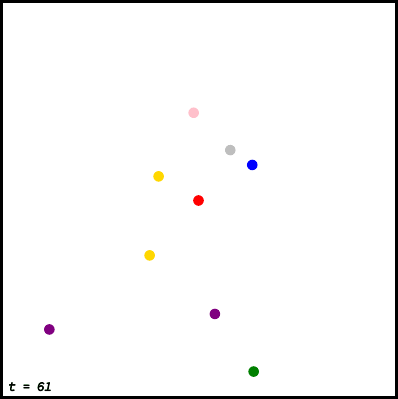
\includegraphics[width = 0.5\textwidth]{images/n-body.png}\\[1.0 cm]	% University Logo
	\textsc{\Large \theauthor}\\[0.5 cm]				% Course Code
	\rule{\linewidth}{0.2 mm} \\[0.4 cm]
	{ \huge \bfseries \thetitle}\\                  
	\rule{\linewidth}{0.2 mm} \\[1.5 cm]
    % \theauthor
    \thedate\\
\end{titlepage}

%%%%%%%%%%%%%%%%%%%%%%%%%%%%%%%%%%%%%%%%%%%%%%%%%%%%%%%%%%%%%%%%%%%%%%%%%%%%%%%%%%%%%%%%%
\section{Introduction}
The N-body problem \cite{wiki:N-body_problem} is a well-known problem in physics that concerns the interactions between multiple bodies under the presence of a specific class of attraction force that includes gravitational or electrostatic force. 
Interestingly, it does not have a general analytical solution for $N \geq 3$, hence the solution to this problem is generally estimated using computational simulation, called N-body simulation \cite{wiki:N-body_simulation}.

To put it formally, we want to predict the trajectories $\boldsymbol{r}_i(t)$ \footnote{To distinguish between scalars and vectors types, we will denote vectors in \textbf{bold}} of $N$ bodies in space.
Each body has an inherent coefficient $\lambda_i$ (e.g. mass or electric charge) which is constant in time.
The force acting by body $j$ on body $i$ is of the form:
$$\boldsymbol{F}_{i \gets j} = \alpha \frac{\lambda_i \lambda_j}{\|\boldsymbol{r}_i - \boldsymbol{r}_j\|^3} (\boldsymbol{r}_j - \boldsymbol{r}_i)$$
where $\alpha$ is some constant (e.g $G$ for gravitational force or $-(4\pi\varepsilon\varepsilon_0)^{-1}$ for electrostatic force), and $\boldsymbol{r}_k$ is the vector representing its position in the space.

By the principle of superposition, the net force on body $k$ is the sum of all forces from all other bodies, and by Newton's second law, 
$$\frac{d^2}{dt^2} \boldsymbol{r}_i(t) 
= \frac{\boldsymbol{F}_i}{m_i} 
= \frac{1}{m_i} \sum_{j \neq i} \boldsymbol{F}_{i \gets j}
= \frac{\alpha \lambda_i}{m_i} \sum_{j \neq i} \frac{\lambda_j}{\|\boldsymbol{r}_i - \boldsymbol{r}_j\|^3} (\boldsymbol{r}_j - \boldsymbol{r}_i)$$
where $m_i$ is the mass of body $i$.

In this report, we will mainly consider the case of gravitational force, so that $\alpha = G$ and $\lambda_i = m_i$. Other types of n-body simulations can be obtained by extending the formula. For simplicity, we will also restrict our scope to the 2-d case, and represent the system in the Cartesian coordinate with $x$ and $y$ axes.

Let us also briefly talk about the complexity of this problem - after all, runtime is a great concern behind the field of parallel computing. The complexity has two major parts: the number of steps and the work per step. 

In order to reduce the number of steps, we can choose a more accurate computing scheme. For example, the leapfrog scheme that is used in this project is of order 2, meaning the error $\varepsilon = O(dt^2)$. There are other schemes that are of different order such as the Euler scheme, which is very similar to the leapfrog scheme but is of order 1 ($\varepsilon = O(dt)$), or the Runge-Kutta 4 scheme of order 4 ($\varepsilon = O(dt^4)$), yet is more difficult to implement.

Regarding the work per step, we will explore two main ideas in this project: the Naive simulation and the Barnes-Hut simulation. The Naive simulation is done by calculating the interaction between all pairs of bodies, which results in a complexity of $O(n^2)$. The Barnes-Hut algorithm sacrifices the error in order to achieve a better complexity of only $O(n \log n)$.

\section{A simple algorithm}
We will restrict our scope to the Leapfrog \cite{wiki:Leapfrog_integration} integration scheme, which is described as follows:

\begin{algorithm}
\caption{Leapfrog}
\KwData{$N$ (the number of bodies)}
\KwData{$dt > 0$ (the time step), $t_{end} > 0$ (the simulation period)}
\KwData{$\boldsymbol{r[N]}(0)$ (an array of size $N \times d$ containing the original positions}
\KwData{$\boldsymbol{v[N]}(-dt/2)$ (an array of size $N\times d$ containing the original velocities}

$t\gets 0$\;
\While{$t < t_{end}$} {
    Calculate $\boldsymbol{F}(t)$ \\
    $\boldsymbol{v}(t + dt/2) = \boldsymbol{v}(t-dt/2) + \boldsymbol{F}(t) / m \times dt$\\
    $\boldsymbol{r}(t + dt) = \boldsymbol{r}(t) + \boldsymbol{v}(t+dt/2) \times dt$\\
    $t\gets t + dt$\
}
\end{algorithm}

This scheme has the advantage of being easy to implement, is of order two, and is also time-reversible. By using the scheme of order two, the error should be of order $O(dt^2)$ so that we can use a larger $dt$ in order to obtain the same error. In addition, the time-reversible property guarantees that the energy is conserved, unlike higher-order schemes like Runge-Kutta 4 (RK4). This means that for large time intervals, we will obtain a more realistic simulation compared to RK4. There are also improvements to the Leapfrog scheme to make it of order 4, but since it introduces much complexity to the code, we have decided not to focus on this but instead on the parallelization aspect.

We can then implement the scheme in a straightforward single-threaded manner: At each time step, we compute the force of all pairs $(i, j)$, then update $\boldsymbol{v}$. Once the updates to $\boldsymbol{v}$ are done, we update $\boldsymbol{r}$. Since $\boldsymbol{F}_{i \gets j} = -\boldsymbol{F}_{j \gets i}$, we could cut the force calculation by half. The algorithm is implemented in \verb|single_thread| function.

\section{A simple GUI to visualize the result}
In order to visualize the result, we have also implemented a function using Magick++ to export the state to a GIF format. We wrap this function inside a \verb|Drawer| object, which manages a thread to draw the frame from the current state independently of the main algorithm. This \verb|Drawer| exposes a \verb|trigger_draw| function that waits for the current drawing thread to finish before copying the current state into its internal buffer and starting the thread again. The internal buffer allows the \verb|Drawer| to operate in parallel with the main algorithm. We have included several examples in the Gallery section of the GitHub repository \ref{sec:repo}.

\section{Parallelizing the algorithm}
Having done the single-thread algorithm and the parallel GUI, the next step is to make our single-thread algorithm multi-threaded. A first idea would be that the velocity update stage and the position update stage can both be parallelized. We can thus distribute the bodies among the threads, and each thread will update its associated bodies. 

Since the force is dependent on the current position, we need to wait for all the velocity updates to finish before updating the positions. This means we need to spawn threads twice for each time step. Going a step further, if we use an alternate buffer to store the updated position, we could make the threads update both the velocity and then the position. This means we only need to spawn threads once per time step, and the overhead of thread creation is mitigated. This multi-threaded version (named \verb|multi_thread_1| yields a speed-up over the single-threaded version of 1.5, 2.63, and 3.8 when run with 2, 4, and 6 parallel threads respectively.

However, a current drawback of this algorithm is that it computes $\boldsymbol{F}_{i\gets j}$ twice, once for each $i^{th}$ and $j^{th}$ bodies. While the whole update step could be done parallelly, each thread can only update its own bodies, hence we can only avoid double computation between bodies inside the same group. In order to mitigate this, an approach (named \verb|multi_thread_2|) would be to split $\boldsymbol{F}_i$ into $\boldsymbol{F}_i^k$ components, one for each thread. Once the parallel force computation is done, the main thread will gather this result and perform the necessary update (in a synchronous manner). While this means that part of the computation cannot be parallelized, the synchronous part is only $O(n)$, while we have cut the $O(n^2)$ by half. We further optimized this approach so that each thread is given a similar load, which results in roughly 1.5 speed-up for 6 parallel threads over the previous multi-threaded version.



\section{Moving on to Barnes-Hut}
The Barnes-Hut algorithm \cite{wiki:Barnes–Hut_simulation} is a hierarchical algorithm that uses a quadtree to approximate the forces between bodies in the n-body simulation. This algorithm has a complexity of $O(n\log n)$ and is hence, faster than the simple Leapfrog algorithm used above which has a complexity of $O(n^2)$. It is important, however, to note that this complexity also depends on the parameter $\theta$. Choosing $\theta = 0$, for example, results in a complexity of $O(n^2)$.

The idea of the algorithm is relatively simple. The algorithm iterates over all the bodies in the simulation and assigns them unique nodes in the quadtree recursively. When a new body is added to the quadtree, the center of mass of every parent node of the quad node where the body is added is updated. Once the quadtree is created, the algorithm computes the force $\boldsymbol{F}_{i \gets j}$ of all bodies $j$ on body $i$ where $(j \neq i)$. In this computation though, we introduce the parameter $\theta$ that is used to compare the ratio $\frac{s}{d}$ where $s=$ \{distance of the body $i$ from the center of mass of the quad $j$\} and $d=$ \{width of the quad\}. In our case, we took $\theta=0.5$. So, if let's say for a certain quad $k$, $\frac{s_{ik}}{d_k} < \theta=0.5$, then all the bodies in the quad $k$ are close enough to the body $i$ to have a significant individual impact on the force they exert on body $i$ and hence we iterate recursively through the children nodes of the quad to compute their individual forces with respect to the body $i$. If, on the other hand, $\frac{s_{ik}}{d_k} \geq \theta=0.5$, then we assume that the center of mass of the bodies in the quad is far enough from the body $i$ and instead of iterating through the children of that quad node we may directly compute the force $\boldsymbol{F}_{i \gets k}$ of the center of mass of the quad $k$ with the body $i$ without having any adverse effect on the overall force computation while also reducing the time taken for it.

In our implementation of the algorithm, we have the following elements:
\begin{itemize}
    \item The \verb|QuadNode| class represents a node in the quadtree. It contains the information for its center, dimension, the overall scenario of all bodies, the mass of the bodies is contained, the center of mass of the bodies, the id of those bodies, and references to its four children nodes. The class also contains methods to construct the quadtree and helper functions as required.
    \item The \verb|addBody| function is used to construct the quadtree by recursively adding each new body in a unique node in the tree. In the recursion though, we check if the dimension of the current node is less than $10^{-3}$ and if it is so, we do not recurse further and instead simply merge the bodies in the quad into a single body by updating its overall mass and the center of mass. This is done to prevent an infinite recursion where two randomly generated bodies might only be nanometers apart or even overlap.
    \item The \verb|barnes_hut_update_step| function computes the forces acting on each body in relation to every quad node of the tree and then updates the velocity of each body for the current timestep in the overall scenario.
\end{itemize}

\section{Parallelizing Barnes-Hut}

The \verb|Barnes-Hut| algorithm essentially works in two steps, in the first it creates the quadtree for all the bodies in the current \verb|Scenario|, and then it calculates the force exerted by each body on every other body or center of mass in the case of approximation. For parallelizing the algorithm, we would have to parallelize these two steps separately as they are independent. 
\begin{itemize}
    \item For parallelizing the construction of the quadtree, we decided not to do so because of its inherent limitations. Let's assume for instance that we parallelize the construction of the quadtree. Then, it is possible that two threads are spawned such that both of them want to add a body in the same quad node and hence recurse into the same quad node which would be susceptible to race conditions. To avoid this, we can assign a thread to a specific quad of the tree and if a body is added to that quad, then the recursion will be handled by the thread responsible for the quad. In this case, though, we are limited by the number of threads. We only have a finite number of threads and these would be hardcoded for every quad. Further, the worst-case complexity of the creation of the quadtree will remain the same as that of the unparalleled version if all bodies are present in a single quad node. Moreover, the overhead of spawning threads in every timestep of the algorithm makes the parallelization inviable.
    \item For the second part, we decided to parallelize the force calculation on each body by dividing the total number of bodies into equal chunks and passing them separately into each thread. Essentially, in this case, the quadtree remains constant and there is no conflict or possibility of race condition in calculating the force on the bodies because the force calculated on each body is handled by a specific thread only. Once the force is calculated, we update the positions of the bodies in a single loop which takes $O(n)$ and this step cannot be included in the parallelized code as it may lead to race conditions. On the other hand, parallelizing this updation step individually is not very useful as we will not save enough time compared to the overhead costs of spawning and joining the threads.
\end{itemize}

\section{Results}

\begin{figure}[hbt!]
    \centering
    \begin{subfigure}[b]{0.32\textwidth}
        \centering
        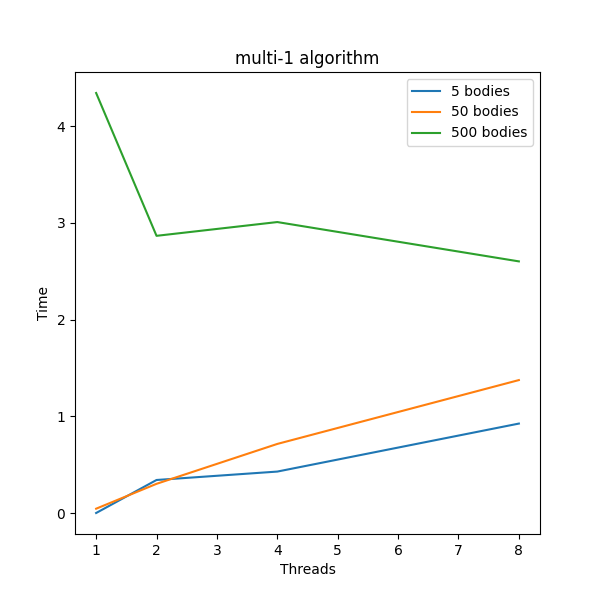
\includegraphics[width=\textwidth]{simulation/thread_algo_multi-1.png}
        \caption{Multi-1}
        \label{figure:multi-1-algo}
    \end{subfigure}
    \hfill
    \begin{subfigure}[b]{0.32\textwidth}
        \centering
        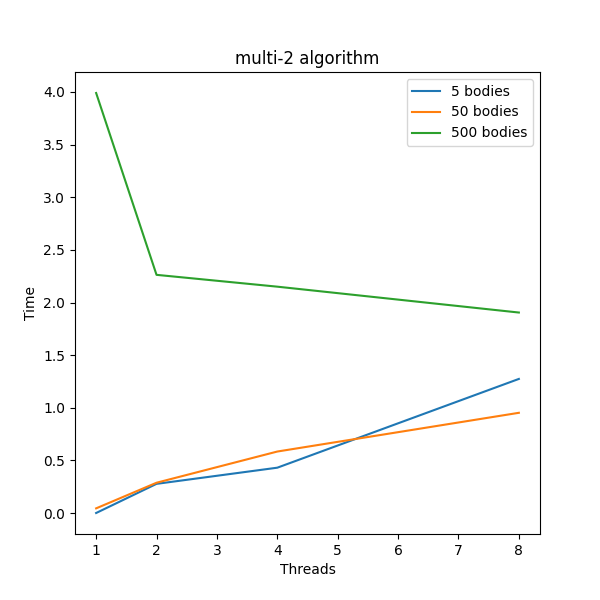
\includegraphics[width=\textwidth]{simulation/thread_algo_multi-2.png}
        \caption{Multi-2}
        \label{figure:multi-2-algo}
    \end{subfigure}
    \hfill
    \begin{subfigure}[b]{0.32\textwidth}
        \centering
        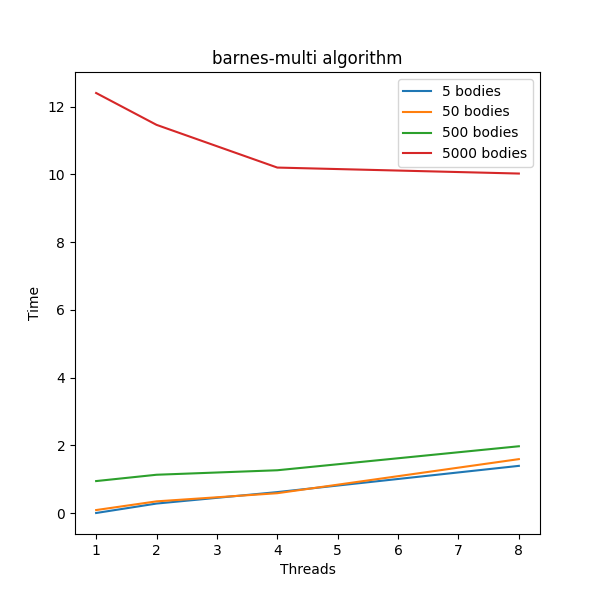
\includegraphics[width=\textwidth]{simulation/thread_algo_barnes-multi.png}
        \caption{Barnes-Hut multi}
        \label{figure:barnes-hut-algo}
    \end{subfigure}
    \caption[hmm]{The graphs compare the running time of the three multi-threaded algorithms compared with the number of threads used for the calculations.}
    \label{figure:thread_algo}
\end{figure}

\begin{figure}[hbt!]
    \centering
    \begin{subfigure}[b]{0.41\textwidth}
        \centering
        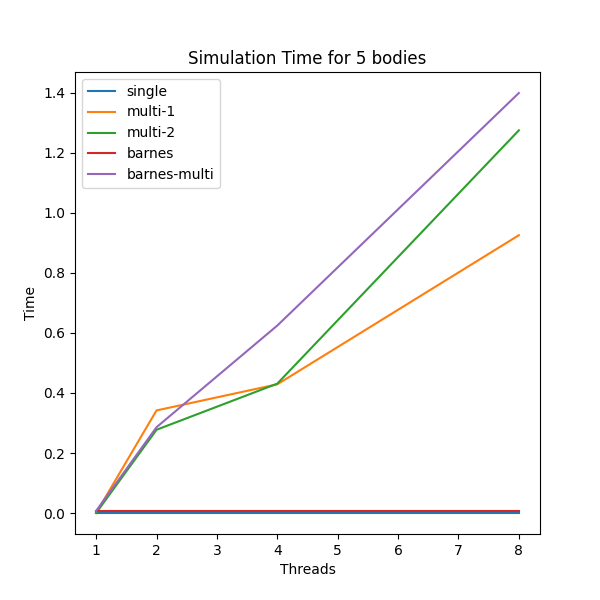
\includegraphics[width=\textwidth]{simulation/simulation_time_5.png}
        \caption{5 body simulation}
        \label{figure:5-body}
    \end{subfigure}
    \hfill
    \begin{subfigure}[b]{0.41\textwidth}
        \centering
        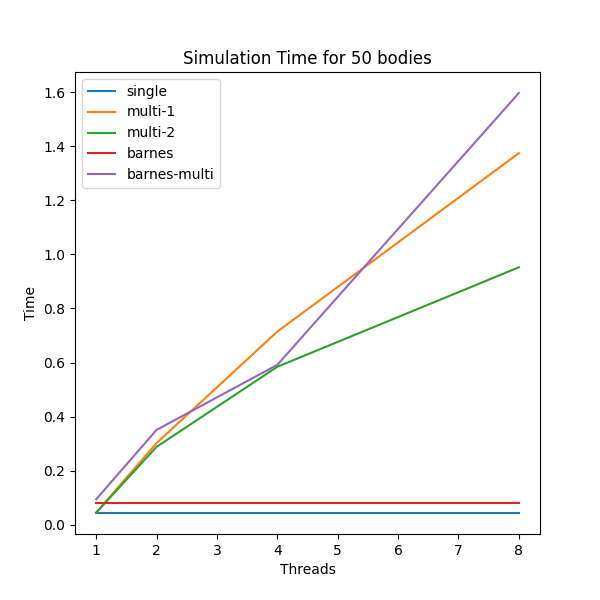
\includegraphics[width=\textwidth]{simulation/simulation_time_50.png}
        \caption{50 body simulation}
        \label{figure:50-body}
    \end{subfigure}
    \hfill
    \begin{subfigure}[b]{0.41\textwidth}
        \centering
        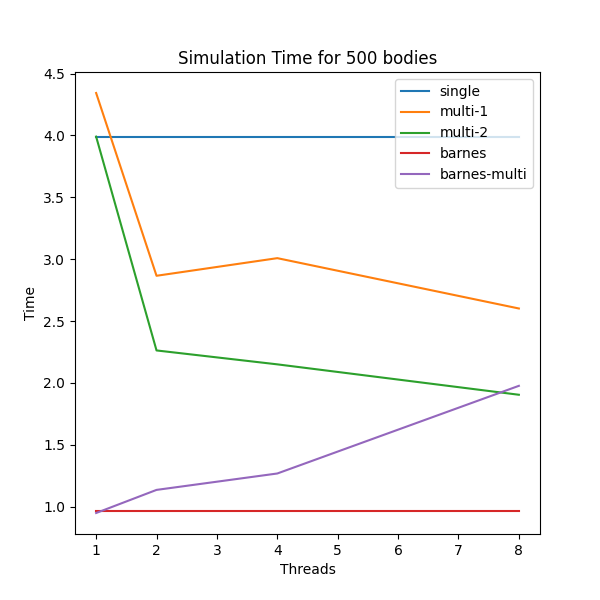
\includegraphics[width=\textwidth]{simulation/simulation_time_500.png}
        \caption{500 body simulation}
        \label{figure:500-body}
    \end{subfigure}
    \hfill
    \begin{subfigure}[b]{0.41\textwidth}
        \centering
        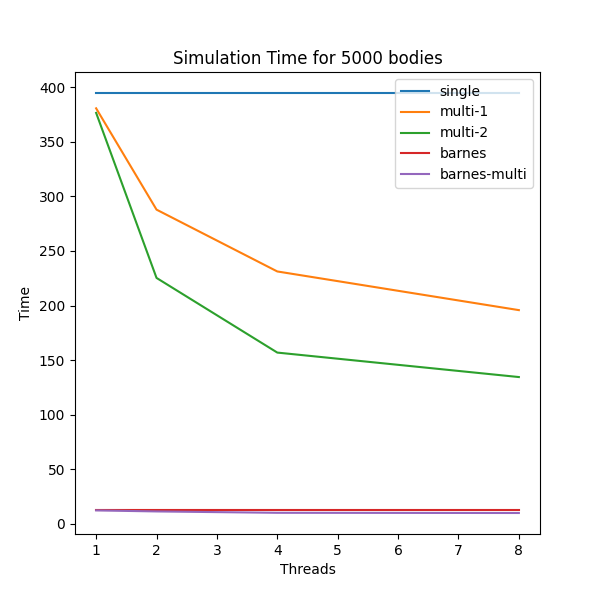
\includegraphics[width=\textwidth]{simulation/simulation_time_5000.png}
        \caption{5000 body simulation}
        \label{figure:5000-body}
    \end{subfigure}
    \caption[hmm]{Simulation runtime with respect to the number of threads for all 5 implemented algorithms. The graphs were plotted using numpy\footnotemark and matplotlib \footnotemark}
    \label{figure:n-body}
\end{figure}
\footnotetext[2]{\url{https://numpy.org/}}
\footnotetext[3]{\url{https://matplotlib.org/}}

Table~\ref{table:simulation-time} in Appendix \ref{appendix:table} summarizes the runtime of different algorithms with different numbers of threads, and these results are also plotted in Figure~\ref{figure:n-body} for comparisons.
We tested the algorithms for bodies of sizes $5, 50, 500, 5000$ and $1, 2, 4, 8$ number of threads for all the parallel algorithms. 

We could clearly observe the complexities of the algorithms: The $O(n^2)$ leapfrog scheme runs 100 times slower for 10 times more bodies, while the $O(n \log n)$ Barnes-Hut scheme runs roughly 10 times slower for 10 times more bodies. For smaller numbers of bodies, the leapfrog scheme runs faster than the Barnes-Hut scheme since it does not have the overhead of building the quadtree, and the Barnes-Hut scheme does not make any approximation for a small number of bodies.

Regarding the number of threads, we saw that the multi-threaded leapfrog schemes have a clear speed-up over the single-threaded one for a larger number of bodies since the overhead of spawning threads is outweighed by the actual computation.
The \verb|multi_thread_2| version outperforms the \verb|multi_thread_1| by roughly 1.5 times since it no longer computes the $O(n^2)$ part twice but has to synchronously compute the $O(n)$ part.

The multi-threaded Barnes-Hut only sees a speedup over the single-threaded one at a large number of bodies. This is because it parallelizes a $O(n\log n)$ complexity portion, which means that we need a large $N$ in order for the thread creation overheads to outweigh this computation.

Further, we can make an interesting observation from the graphs in figure \ref{figure:thread_algo}. For the multi-threaded algorithms, we see that for the simulation of the 5-body and 50-body systems, increasing the number of threads actually increases the overall simulation time by roughly two for each of the algorithms. In fact, there is a speed-up compared to the single-threaded implementation only when the system has 500 bodies (for the Barnes-hut it speeds up only for 5000 bodies). This clearly shows that the overhead of spawning and joining the parallel threads does not benefit the overall simulation time and for small n-body systems ($\approx100$) it is better to use the single-threaded version than the multi-threaded implementation of the algorithms.

\section{Error Analysis}

\begin{figure}[hbt!]
    \centering
    \begin{subfigure}[b]{0.49\textwidth}
        \centering
        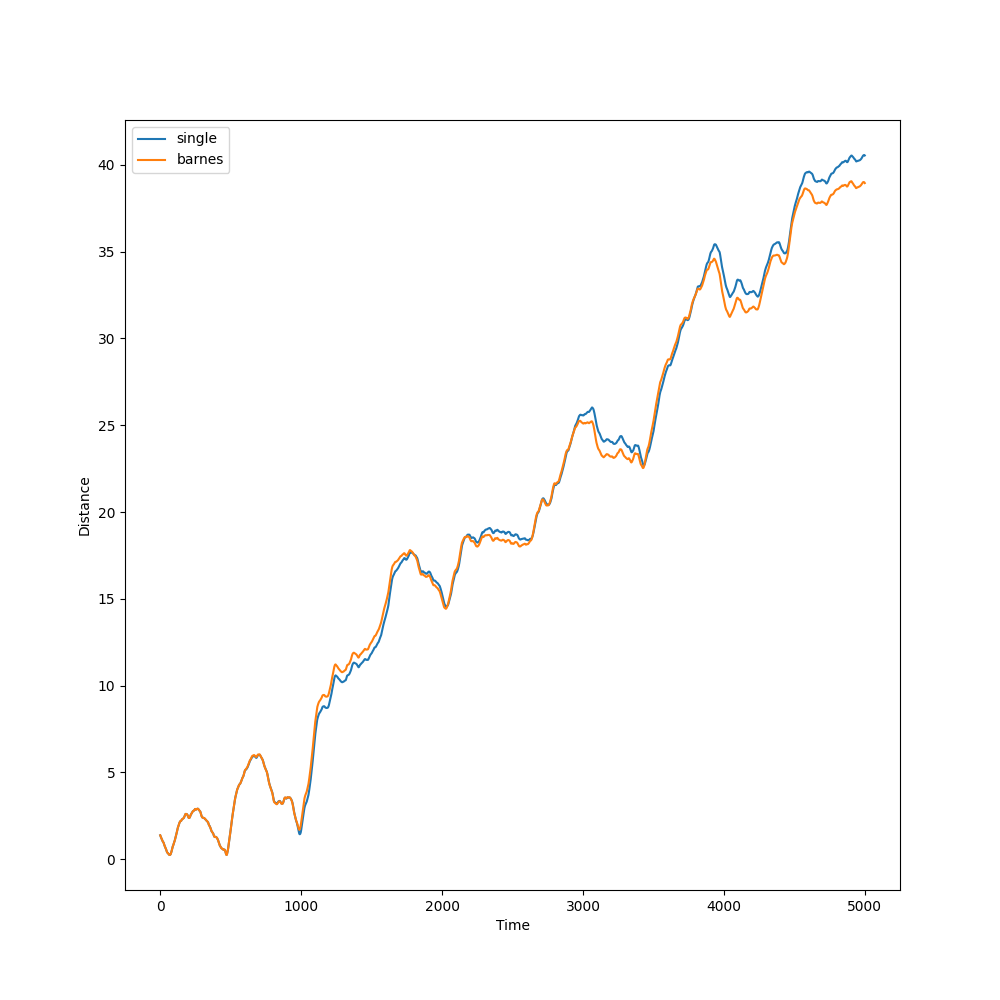
\includegraphics[width=\textwidth]{images/distance.png}
        \caption{Average displacement of a body from the center for the two algorithms}
        \label{figure:trajectory}
    \end{subfigure}
    \hfill
    \begin{subfigure}[b]{0.49\textwidth}
        \centering
        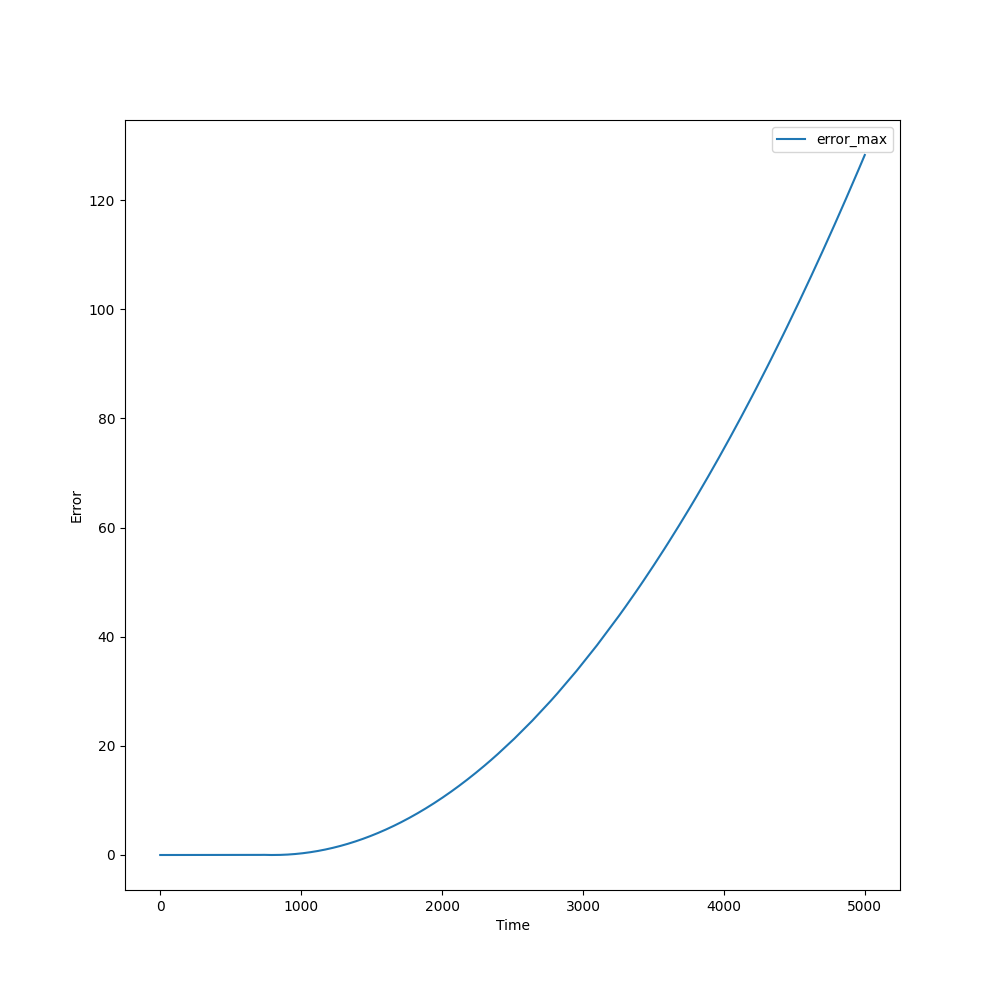
\includegraphics[width=\textwidth]{images/error_max.png}
        \caption{Maximum error in the position of the same body calculated by the two algorithms}
        \label{figure:error-max}
    \end{subfigure}
    \hfill
    \begin{subfigure}[b]{0.49\textwidth}
        \centering
        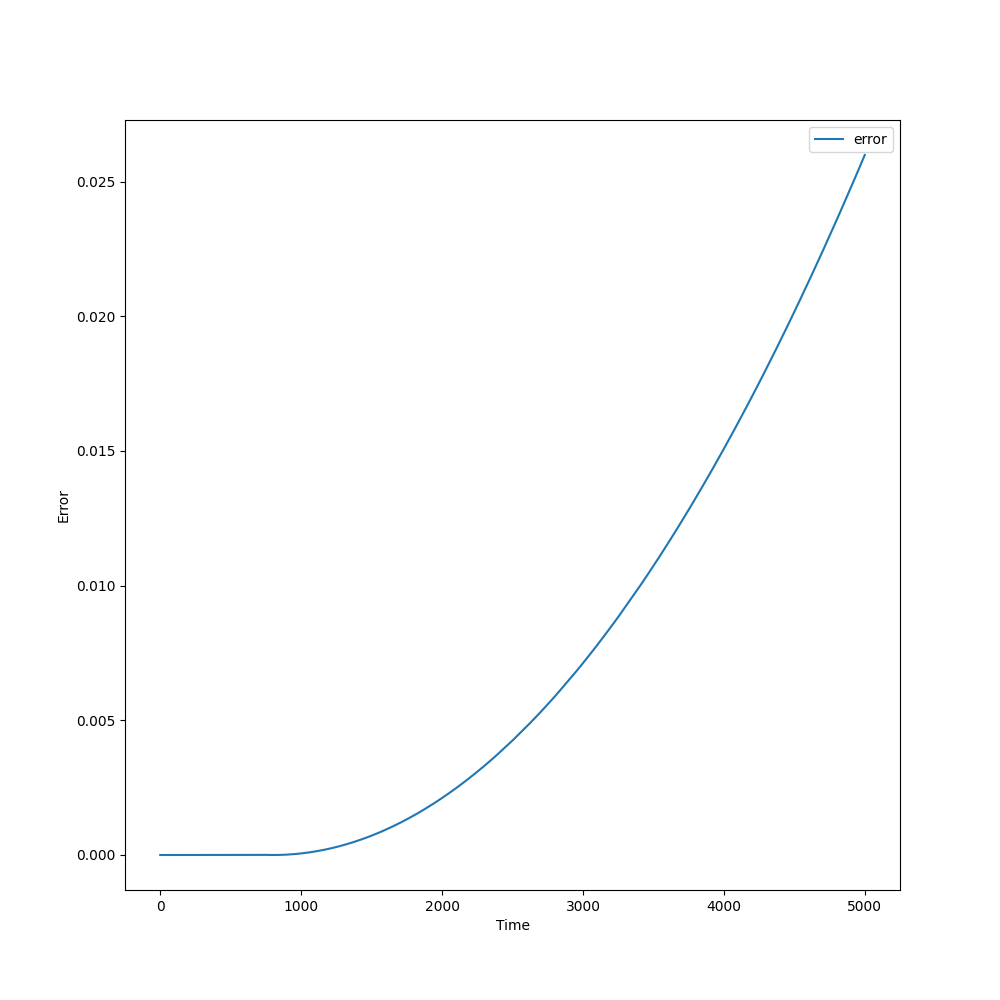
\includegraphics[width=\textwidth]{images/error.png}
        \caption{Average error in the average displacement of a body calculated by the two algorithms}
        \label{figure:error}
    \end{subfigure}
    \caption{Position error analysis for Barnes-Hut and Leapfrog algorithms.}
    \label{figure:power}
\end{figure}  

The Barnes-Hut algorithm uses an approximation mechanism and hence is liable to errors in the overall calculated forces acting on each body which should result in a precision error in the positions of the bodies when compared to the positions calculated by the Leapfrog algorithm. Below, we have plotted some graphs to analyze and study this difference and we used $\theta=0.5$ in the Barnes-Hut algorithm. For the graphs, we first stored the values of the positions of all bodies at each time step from both algorithms in a \verb|.txt| file and then used \verb|matplotlib| to plot them. The code is available in the repository.

In figure \ref{figure:trajectory} we have plotted the average distance of a body from the center of the canvas for 1000 bodies over 5000 timesteps for both the Barnes-Hut and Leapfrog algorithms. In this graph, we can clearly see that over time, the average displacement of a body from the center for the Barnes-Hut algorithm starts to differ as the approximation introduced by it accumulates. This difference can be seen in figure \ref{figure:error} where the average error of the difference between the average position of a body calculated by the two algorithms starts to increase over time. It is also important to note that this error is accumulated in each iteration which results in a non-linear graph for the overall error. Further, figure \ref{figure:error-max} suggests that because the maximum error between the position calculated by the two algorithms for the same body is relatively large, the average error between the position of bodies between the algorithms is probably dominated by only a handful of bodies. This is possible when some bodies are positioned in such a manner that the force acting on them is approximated in each iteration and resultantly their estimated position keeps on diverging from the original one.

\section{Conclusion}
In this project, we have explored two different algorithms for N-body simulation.
The leapfrog scheme has complexity $O(n^2)$, but we could achieve a 2-4 speedup by parallelizing the computation using 2-8 threads.
The Barnes-Hut algorithm, on the other hand, sacrifices the accuracy in order to gain a $O(n \log n)$ complexity. This effect could be observed clearly in the case of 5000 bodies, where this takes a roughly 30 times speedup over the single-threaded leapfrog scheme. However, this comes with the cost of error in the scheme. As observed in Fig~\ref{figure:error} and Fig~\ref{figure:error-max}, this error increases exponentially since it accumulates across time. However, by considering a smaller time step, we could make this error term negligible in order to obtain a fast N-body simulation scheme.


\section{Source code} \label{sec:repo}
The source code of this project is available at \url{https://github.com/nhat-vo/n-body-simulation}, along with instructions on how to build and run.

\appendix
\section{Simluation times for different bodies and threads for the algorithms}
\label{appendix:table}
\begin{table}[htb]
\centering
\begin{tabular}{ |c|c|c|c|c|c| } 
 \hline
 \multirow{2}{8em}{\centering Algorithm}
 & \multirow{2}{4em}{\centering Num. bodies} & \multicolumn{4}{c|}{\centering Num. threads} \\
 \cline{3-6}  
 & & 1 & 2 & 4 & 8\\ 
 \hline
 \multirow{4}{8em}{\centering single-thread} 
 & 5 & 0.000315189s & N/A & N/A & N/A \\ 
 & 50 & 0.0435316s & N/A & N/A & N/A \\ 
 & 500 & 3.98902s & N/A & N/A & N/A \\ 
 & 5000 & 394.694s & N/A & N/A & N/A \\ 
 \hline
 \multirow{4}{8em}{\centering multi-thread-1} 
 & 5 & 0.000408565s & 0.341722s & 0.428695s & 0.924966s \\ 
 & 50 & 0.0448995s & 0.302086s & 0.714518s & 1.37461s \\ 
 & 500 & 4.3428s & 2.86613s & 3.00847s & 2.60183s \\ 
 & 5000 & 380.657s & 287.875s & 231.248s & 195.832s \\ 
 \hline
 \multirow{4}{8em}{\centering multi-thread-2} 
 & 5 & 0.000544892s & 0.277382s & 0.430944s & 1.27411s \\ 
 & 50 & 0.0446863s & 0.288029s & 0.584391s & 0.952332s \\ 
 & 500 & 3.99018s & 2.26284s & 2.15047s & 1.90481s \\ 
 & 5000 & 376.485s & 225.332s & 156.944s & 134.536s \\ 
 \hline
 \multirow{4}{8em}{\centering barnes-hut-single} 
 & 5 & 0.0068054s & N/A & N/A & N/A\\ 
 & 50 & 0.0816349s & N/A & N/A & N/A \\ 
 & 500 & 0.963767s& N/A & N/A & N/A \\ 
 & 5000 & 12.4607s & N/A & N/A & N/A \\
 \hline
 \multirow{4}{8em}{\centering barnes-hut-multi} 
 & 5 & 0.00728977s & 0.285864s & 0.624284s & 1.39838s \\ 
 & 50 & 0.0940806s & 0.350851s & 0.591455s & 1.5971s \\ 
 & 500 & 0.949498s & 1.13613s & 1.2687s & 1.97693s \\ 
 & 5000 & 12.4022s & 11.4622s & 10.2015s & 10.0252s \\ 
  \hline
\end{tabular}
\caption{Total runtime of different algorithms (without any visualization) using different numbers of threads and bodies. 
The results were obtained for 5000 time steps on a machine that uses 11th Gen Intel(R) Core(TM) i5-1135G7 @ 2.40GHz with 8 logical processors.
Note that, since the operating system very probably not dedicate all the cores to the calculations, there would be a certain discrepancy between the actual and expected runtime.
}
\label{table:simulation-time}
\end{table}

\newpage
\printbibliography



\end{document}